\chapter[SCP-021 栖肤龙纹]{
    SCP-021 Skin Wyrm\\
    SCP-021 栖肤龙纹
}

\label{chap:SCP-021}

\begin{figure}[H]
    \centering
    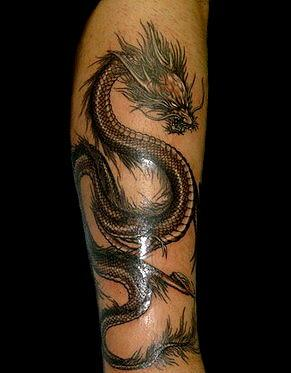
\includegraphics[width=0.5\linewidth]{images/SCP.021.jpg}
    \caption*{SCP-021于实验体D-124(已故)}
\end{figure}

\bb{项目编号:} SCP-021

\bb{项目等级:} Safe

\bb{特殊收容措施:} SCP-021为人体专性寄生物,因此其收容难度并不大于对成年人类的收容难度,大多数密闭房间都满足要求。样本当前寄生于D-139并拘留于217-A。只有D级人员适于成为SCP-021的宿主。当一位D级人员成为SCP-021的宿主时,他应在每月初的例行处决中得到豁免。

\bb{描述:} SCP-021会覆盖宿主大约0.8平方米的皮肤,看上去如同纹身,外观为一条巨大、精致的东方神话体系的蛇形龙。在其所寄宿的皮肤之内,虽然只存在于两个维度,但该纹身完全是活的并表现出普通动物的行为模式。纹身的活动会给宿主带来持续的疼痛,近似于大规模的纹身和纹身移除同时进行。该寄生物一生中的大部分时间都花费在宿主躯干表面或附近。SCP-021并没有表现出觅食和移动之外的智能,然而,对二维空间生命形态的智力测量到目前为止是不可能的。

SCP-021表现出针对宿主皮肤表面色素的单一食性。它可以食用黑色素并导致宿主不得不承受白癜风之苦。但是该寄生物表现出对其他纹身显著偏爱,比起其它自然色素,它会优先找出并吞食宿主体表的纹身。值得注意的是,当不进行移动时,这一进食过程是无痛的。普通的纹身墨水会简单地消失如同被“吃掉”,寄生物维持其体量不变,没有排泄物被观测到。该寄生物每小时可以清理0.6平方米的纹身。“喂食”SCP-021的一个办法是在宿主体表(快速地)纹上水果或小动物图案。

SCP-021可以通过多种物理接触形式来转换到另一个宿主。在一次成功的转移中,寄生物从一个人体表“游”到另一个人体表。性行为是最可靠的转换方式,有高达93\%的成功率。然而,考虑到这一过程会带来的剧烈疼痛,这并不是理想的方式。两人分别以一处开放的伤口互相接触来构成连接是一种更为合理的方式。在已故实验体身上进行转移则更为复杂:虽然并不合情理,但寄生体似乎并未因宿主的死亡而受到不良影响,依然持续进食其体表的色素。不同物种间的转换情况目前未知:既有的实验表明,这种转换要么根本不可能,要么则十分稀少。

SCP-021会对其宿主带来少许益处。已被证明,它会提升肾上腺素的释放和吸收水平,并减少乳酸的生成,从而促进宿主在应激状况中的爆发力、自信和痛苦忍受能力,并减少通常存在的虚弱和疲乏的后遗症。此外,它有可能在某种程度上有益于宿主的免疫系统。宿主的攻击性行为模式概率高于平均水平,这一现象究竟是该纹身的直接影响,或者是其所造成的持续疼痛带来的反应,还有待观察。

这种共生关系的持续时间,一般取决于宿主能忍耐日常生活中持续不断的痛苦到什么程度。已有一定数量的实验体以自杀告终。在极稀少的情况下,宿主最后以致命性皮肤传染病告终。

SCP-021的起源和自然形态依然成谜。在保密的前题下追踪它在一个个宿主之间的传递过程十分困难,并且该寄生物已存在了数百年或更久。然而虽然如此,SCP-021是基金会保管时间最久的项目,已有[资料删除]年之久,并在这段时间里一直有其教育意义。最近对它的研究工作主要集中于观测二维空间内的生物特性。
